%\begin{document}
\chapter{基于先验信息MMSE准则的线性Turbo均衡算法}
\thispagestyle{empty}
%=========================================================================
\section{卷积码与水声通信}
现实中已经开始运用卷积码在水声通信中,而且可以很好的解决误码率问题,但是基于以下分析我们还是要继续研究卷积码的编译码。

由于先前的卷积码采用的是$(4,1,7)$,译码方式自然采用的是维特比译码算法,误码率曲线没什么说的,译码算法效率也是非常出色,但是有个致命的问题,就是码率$R=\frac{1}{4}$,这对于原本带宽就非常狭窄的水声通信系统来说无疑是雪上加霜,因此我们开始关注于卷积码的另外一种译码算法就是序贯译码算法。

序贯译码和维特比译码比较图\cite{Digital_communications}可知,在约束长度$K=41$,码率$R=\frac{1}{2}$的情况下的序贯译码的误码率要比约束长度$K=7$,码率$R=\frac{1}{3}$的维特比译码,软硬判决都好,因此选择序贯译码,可以提高码率。

至于约束长度问题,由于序贯译码的运算量和运行时间与约束长度无关,因此可以选择很大的约束长度,而维特比译码却不可以,这在后面章节会详细介绍。
\section{卷积码概述}
卷积码最早是1955年由伊利亚斯(P.Elias)提出来的。它是一种非分组码,卷积码更适合用于前向纠错法。

在一个二进制分组码$(n,k)$当中,包含$k$个信息位,码组长度为$n$,每个码组的$(n-k)$个校验位仅与本码组的$k$个信息位有关,而与其它码组无关。为了达到一定的纠错能力和编码效率$(R_e=\frac{k}{n})$,分组码的码组长度$n$通常都比较大。编译码时必须把整个信息码组存储起来,由此产生的延时随着$n$的增加而线性增加。

与分组码不同,卷积码中编码后的$n$个码元不仅与当前段的$k$个信息有关,而且也与前码$(N-1)$段的信息有关,编码过程中相互关联的码元为$nN$个。因此,这$N$时间内的码元数目$nN$通常被称为这个码的约束长度。卷积码的纠错能力随着$N$的增加而增大,在编码器复杂程度相同的情况下,卷积码的性能优于分组码。另一点不同的是:分组码有严格的代数结构,但卷积码至今尚未找到如此严密的数学手段,把纠错性能与码的结构十分规律地联系起来,目前大都采用计算机来搜索好码。
%=========================================================================
\section{卷积码的编码\cite{ioa_communications}}
卷积码的编码器是由一个有$k$个输入位、$n$个输出位,且具有$m$级移位寄存器所构成的有限状态的有记忆系统,通常称为时序网络。卷积码编码原理图如图\ref{fig:3.1}
\begin{figure}[htb]
  \begin{center}
    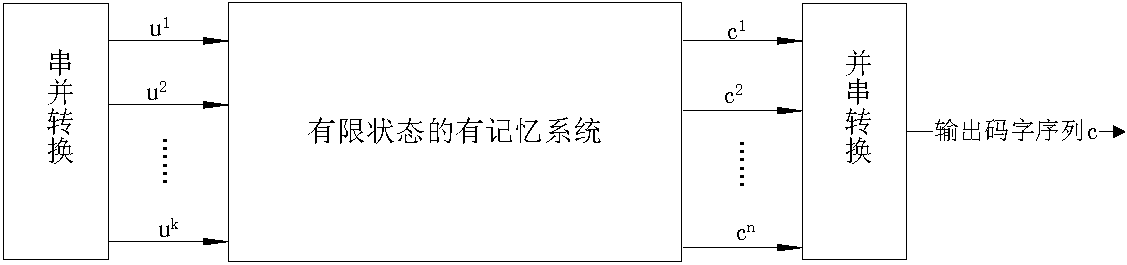
\includegraphics[width=0.8\textwidth]{images/conv1.pdf}
  \end{center}
  \caption{卷积码编码器原理图}
  \label{fig:3.1}
\end{figure}
表\ref{tab:3.1}给出了卷积码一些参数及其说明。
\begin{table}[hbp]
  \centering
  \caption{卷积码编码器参数}
  \label{tab:3.1}
  \begin{tabular}{|l|}
    \hline 
  \begin{minipage}[tb]{15cm}
    \vspace{5mm}
    \textbf{\sanhao 卷积编码器的记忆参数\cite{Coding_Theory}}
      \begin{itemize}
        \item
          $k$和$n$分别表示编码器输入和输出位。编码效率为$R=\frac{k}{n}$
        \item 当前$n$位的输出是当前$k$位和前$k\times
          m$位输入的线性组合,这里的$m$称为卷积码的记忆长度。
        \item 二进制卷积码通常用3个参数写成$(n,k,m)$。
        \item 编码器的记忆长度$m=\max_lv_l$。
        \item 最小约束长度$v_{min}=\min_lv_l$。
        \item 总约束长度$v=\sum_{l=1}^{k}v_l$。
      \end{itemize}
      \vspace{5mm}
    \end{minipage}\\
    \hline
  \end{tabular}
\end{table}

描述这类时序网络的方法很多,大致分为两大类型:解析表示法与图形表示法。在解析法中又可分为离散卷积法、生成矩阵法、码多项式法等;在图形表示法中也可分为状态图法、树图法、网格图法等。由于这个设计着重于实现卷积码的编码与序贯译码,所以只介绍码多项式法、状态图法以及网格图法。
下面,引用具体实例对这三种表示方法加以说明。图\ref{fig:3.2}给出一个二元(2,1,3)卷积码的编码器结构。
\begin{figure}[htb]
  \begin{center}
    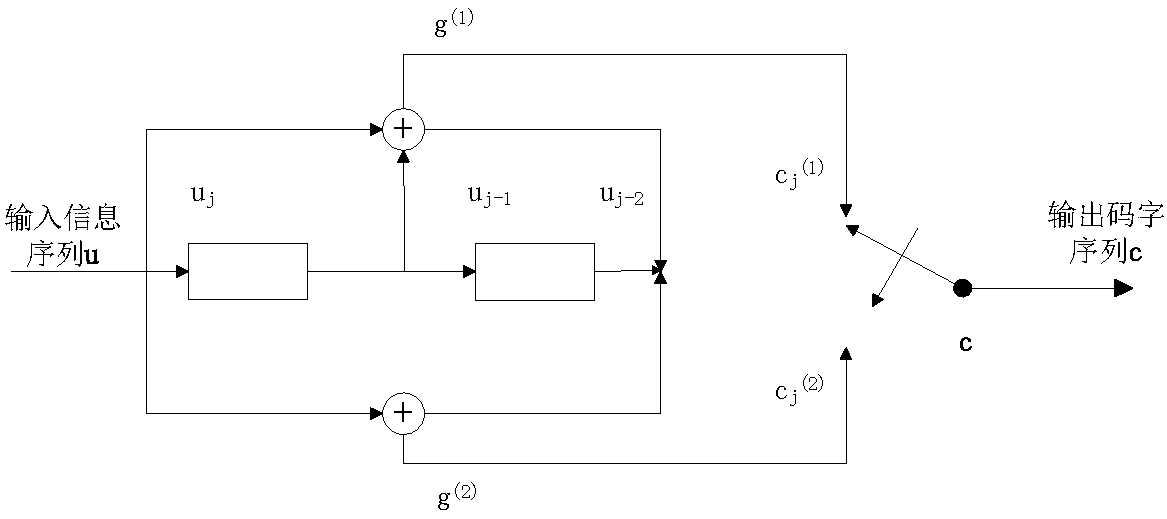
\includegraphics[width=0.8\textwidth]{images/conv2.pdf}
  \end{center}
  \caption{编码效率为1/2,约束长度$K=3$的(2,1,3)卷积码编码器}
  \label{fig:3.2}
\end{figure}
由图可见,它是由$k=1$即一个输入位,$n=2$即两个输出位,$K=3,m=2$即两级移位寄存器所组成的有限状态的有记忆系统。
\subsection{多项式法}
由上图可以看出,该卷积码的生成多项式为
\begin{eqnarray}
  \begin{array}{lll}
    \mathbf{g}^{(1)}~&=&~(111)=1+x+x^2 \\
    \mathbf{g}^{(2)}~&=&~(101)=1+x^2
\end{array}
  \label{equ:3.1}
\end{eqnarray}
输入信息序列也可以表达为多项式(在这里,最左边的比特对应于多项式的最低次项)
\begin{eqnarray}
  \mathbf{u}=(10111)=1+x^2+x^3+x^4
  \label{equ:3.2}
\end{eqnarray}
则卷积码可以用下列码多项式表达
\begin{eqnarray}
  \begin{array}{l@{\mbox{=}}l}
  
    \mathbf{c}^{(1)}&(1+x^2+x^3+x^4)(1+x+x^2)\\
    &1+x^2+x^3+x^4+x+x^3+x^4+x^6+x^2+x^4+x^5+x^6\\
    &1+x+x^4+x^6\\
    &(1100101)\\
    \mathbf{c}^{(2)}&(1+x^2+x^3+x^4)(1+x^2)\\
    &1+x^2+x^3+x^4+x^2+x^4+x^5+x^6\\
    &1+x^3+x^5+x^6\\
    &(1001011)\\
 \end{array}
  \label{equ:3.3}
\end{eqnarray}
所以最终生成的卷积码为$\mathbf{c}=(11100001100100)$。
\subsection{状态图法}
卷积编码器的状态图描述了编码器的运行。在讨论卷积码的距离特性和译码算法时,状态图将非常有用。

由于卷积码编码器在下一时刻的输出取决于编码器当前的状态及下一时刻的输入。而编码器当前状态取决于编码器在当前各移位寄存器所存储的内容,称编码器的各移位寄存器在任一时刻的存数(0或1)为编码器在该时刻的一个状态\footnote{此状态表示记忆着以前的输入信息}。随着信息序列的不断输入,编码器就不断从一个状态转移到另一个状态,并输出相应的码序列。编码器的总可能状态数是$2^{mk}$个。

取图\ref{fig:3.2}所示的卷积码编码器,其状态图如\ref{fig:3.3}所示。
\begin{figure}[htb]
  \begin{center}
    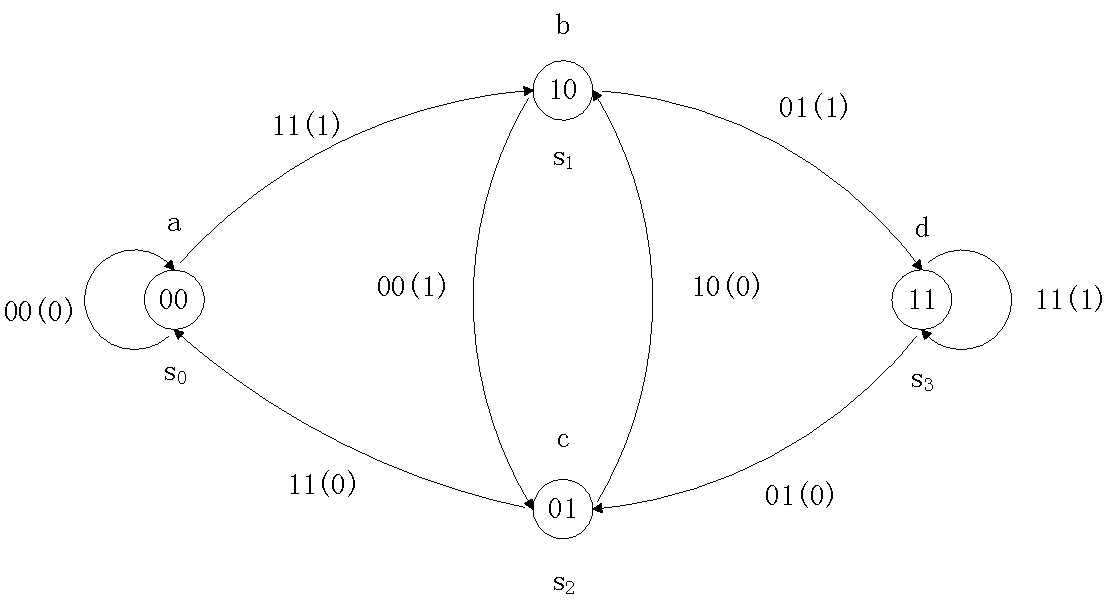
\includegraphics[width=0.6\textwidth]{images/conv3.pdf}
  \end{center}
  \caption{(2,1,3)卷积码状态图}
  \label{fig:3.3}
\end{figure}
图\ref{fig:3.3}中,4个圆圈中的数字表示状态,状态之间的连线与箭头表示转移方向,称作分支,分支上的数字表示由一个状态到另一个状态转移时的输出码字,而括号中数字表示相应的输入信息数字。
\subsection{网格图}
网格图的概念是由Forney提出的。图\ref{fig:3.4}给出了图\ref{fig:3.2}编码器的网格图。该图的纵坐标表示所有状态,横坐标表示时间,节点表示编码器的状态。这类网格图描述法在卷积码的维特比译码和序贯译码中都有很重要的作用,它综合了状态图和树图的优点,即网格图既有状态图结构简单,又具有树图的时序关系清晰特点。
\begin{figure}[htb]
  \begin{center}
    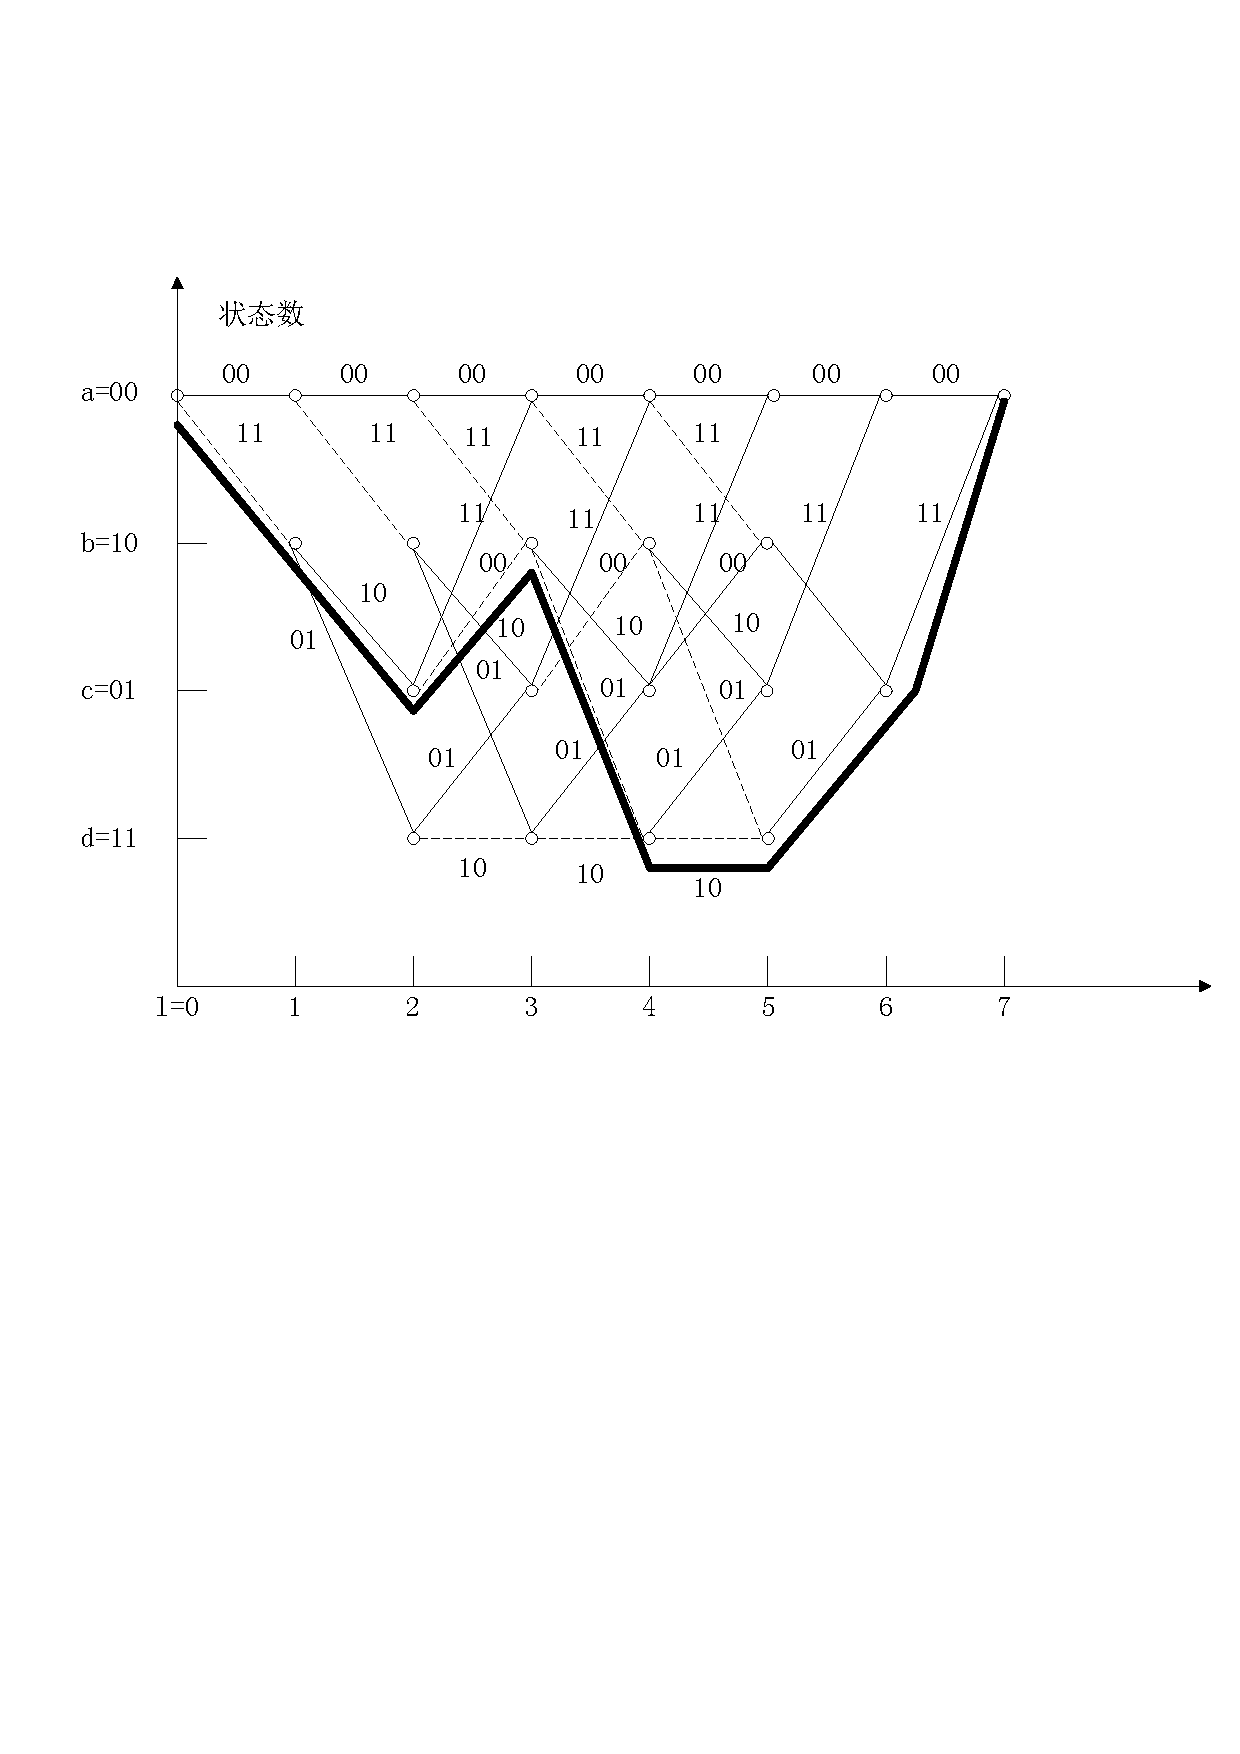
\includegraphics[width=0.6\textwidth]{images/conv4.pdf}
  \end{center}
  \caption{(2,1,3)卷积码网格图表示法}
  \label{fig:3.4}
\end{figure}
图\ref{fig:3.4}中实线表示输入为0时所走的分支,虚线表示输入为1时所走的分支。从网格图中可以看出卷积码编码需要考虑的一个问题,就是码的终结。

理论上卷积码的码序列是无限长的。但是在实际应用中通常都是有限长的码序列。表\ref{tab:3.2}列举了3种获得有限长码序列的方法。
\begin{table}[htb]
  \centering
  \caption{码的终结方法}
  \label{tab:3.2}
  \begin{tabular}{|l|}
    \hline 
  \begin{minipage}[tb]{15cm}
    \vspace{5mm}
    \textbf{\sanhao 码的终结方法\cite{Coding_Theory}}
    \begin{description}
      \item[\textbf{\sanhao
        截断(Truncation):}]在一定数量的比特之后停止编码,不采取任何措施。这会在序列的最后若干比特上导致交大差错概率。
      \item[\textbf{\sanhao
        终结(Termination):}]在码序列后面附加一些尾序列,以保证编码器进入预定的结束状态。这样,序列最后若干比特的差错概率较低。
      \item[\textbf{\sanhao
        咬尾(Tail-biting):}]选用一种起始状态,能保证起始和结束首尾状态相同。这样,序列最后若干比特的差错概率与前面一样。
    \end{description}
      \vspace{5mm}
    \end{minipage}\\
    \hline
  \end{tabular}
\end{table}
结合表\ref{tab:3.2}与实际编译码时候的需要,本设计选择的是终结与咬尾方式的结合,也就是,通过增加一些尾序列使得初始状态和结束状态相同,从而降低最后若干比特的差错概率。
%=========================================================================
\section{卷积码的译码}
卷积码的译码基本上可划分为两大类:代数译码和概率译码。在分组码中一般用代数译码,在RS译码方式中我们将介绍,而这里则侧重介绍概率译码,而且概率译码也是实际中最常采用的卷积码译码方法。

1967年,维特比(Viterbi)引入了一种卷积码的译码算法,这就是著名的维特比算法。后来Omura证明维特比译码等价于求通过一个加权图的最短路径问题的动态规划解。最后Forney指出它事实上就是卷积码的最大似然译码算法,即译码器所选择的输出总是能给出对数似然函数值为最大的码字。

早在维特比译码算法提出之前,已有其它译码卷积码算法,最早的是由Wozencraft提出,后经Fano修改的序贯译码算法(sequential
decoding
algorithm\cite{Error_fano})。序贯译码的工作原理是,对发送码字序列进行假定,计算这些假定序列和接收信号之间的距离度量,只要度量值表明该选择是可能的,就继续译码;否则就向后返回,并改变假设序列,直到通过系统的试验-纠正搜索后找到可能的假设序列。

维特比算法的主要缺陷是,尽管差错概率随着约束长度按指数级减少,但是编码状态数以及相应的译码器复杂性,都随着约束长度呈指数级增长。另一方面,维特比算法的计算复杂性与信道特性无关(和硬判决相比,软判决需要的计算量仅略微增加)。序贯译码渐地达到了和最大似然译码一样的差错概率,但不需要搜索所有的可能状态。实际上,顺序译码所要搜索的状态数,本质上和约束长度无关,因此,可以使用较大$(K=41)$的约束长度。这是提供低差错率的重要因素。序贯译码的主要缺陷是,它搜索的状态量度的数量是一个随机变量。对于序贯译码,不良假设和回溯搜索的个数是信道SNR\footnote{Sound
Noice Ratio
信噪比}的函数。当SNR较低时的假设次数要比SNR较高时多。由于存在这种计算负荷的变化,必须使用缓冲器来存储到达的序列。

由于是水声通信,因此对于运算量的要求比较严,所有维特比译码算法显然就不适合要求,而序贯译码采用约束长度较大时,译码效率不次于维特比译码算法,甚至比它还要好,误码率还要低,而且不需要很多的运算量,至于缓冲区,对于一个水声通信来说不成问题。

综合上面的考虑,选择序贯译码\cite{Anderson_fano}来作为卷积码译码方式。
%===========================================================================
\section{费诺(Fano)算法}
现有的序贯译码算法有两大类:费诺算法和堆栈算法\cite{Geist_fano}。

堆栈算法的最大优点是保存了所有搜索路径从而使搜索效率最高,代价是维持一个过于庞大的堆栈,而费诺算法则正相反,省去了存储器,但是会增加很多计算量。

结合考虑两种方式、使用的卷积码特点以及实际应用情况,选择的是费诺译码算法。
\subsection{费诺算法原理}
\paragraph*{费诺算法介绍\cite{SunJun_fano}}
前面已经说过费诺度量最大的特点就是没有对搜索过的路径进行存储,省去了庞大的堆栈。搜索的前进和回退是有门限值T来控制,算法只沿一条路径搜索,只存储这条路径的度量值,只要被搜索的路径度量值增加,译码器就一直沿这条路径搜索下去,直到度量值明显下降时为止,译码器回退搜索由前面节点分离出去的分支路径,这种回退控制是由改变门限值T来实现的,当向前搜索时,如果获得足够大的度量值增量就收紧(提高)门限值。当回退搜索时,则放松(降低)门限值,这样保持没有一个节点以两次同样的门限值被搜索到\cite{Forney_fano}。
\paragraph*{费诺度量\cite{Han_fano}}
1963年,通过大量的仿真模拟,费诺度量被发现,并随后被费诺用在序贯译码中\cite{ROBERT_FANO},当做典型的路径度量值。

对于在译码树$l$层中的任意路径$v_{(ln-1)}$,费诺度量定义如下:
\begin{eqnarray}
  M(\mathbf{v}_{(ln-1)}|\mathbf{r}_{(ln-1)})=\sum_{j=0}^{ln-1}M(v_j|r_j).
  \label{equ:3.4}
\end{eqnarray}
其中$\mathbf{r}=(r_0,r_1,\cdots ,r_{N-1})$是接收的信号矢量,并且
\begin{eqnarray}
  M(v_j|r_j)=\log_2\left[\frac{Pr(r_j|v_j)}{Pr(r_j)}\right] -R
  \label{equ:3.5}
\end{eqnarray}
是每个比特位的度量值。

由于本设计只针对于硬判决译码器,因此在错误概率为$p$的BSC\footnote{Binary
Symmetric Channel
二进制对称信道}信道中,$Pr(r_j=0|v_j=1)=Pr(r_j=1|v_j=0)=p \mbox{当}0\le j\le
N-1$,当$0<p<1/2$,$v_{(ln-1)}$的费诺度量为
\begin{eqnarray}
  M(\mathbf{v}_{(ln-1)}|\mathbf{r}_{(ln-1)})=\sum_{j=0}^{ln-1}\log_2Pr(r_j|v_j)+\ln(1-R)
  \label{equ:3.6}
\end{eqnarray}
其中$R=\frac{k}{n}$为码率,
\begin{eqnarray}
  \log_2Pr(r_j|v_j) =\left\{
  \begin{array}{l@{,}l}
    \log_2(1-p)&\mbox{当}r_j=v_j;\\
    \log_2(p)&\mbox{当}r_j\neq v_j;
  \end{array}
    \right.
  \label{equ:3.7}
\end{eqnarray}
因此,式\ref{equ:3.5}结合\ref{equ:3.7}并在错误概率为$p$的BSC信道中,可以推导出单个比特位的度量值为:
\begin{eqnarray}
  M(v_j|r_j)=\left\{
  \begin{array}{l@{,}l}
    \log_2(1-p)+(1-R)&\mbox{当}r_j=v_j;\\
    \log_2(p)+(1-R)&\mbox{当}r_j\neq v_j;
  \end{array}
  \right.
  \label{equ:3.8}
\end{eqnarray}
而路径的费诺度量则是从根节点到当前节点比特位度量的和,因此直接套用式\ref{equ:3.4}即可。
而表\ref{tab:3.3}是关于费诺度量的一些说明。
\begin{table}[htb]
  \centering
  \caption{费诺度量的说明}
  \label{tab:3.3}
  \begin{tabular}{|l|}
    \hline 
  \begin{minipage}[tb]{15cm}
    \vspace{5mm}
    \textbf{\sanhao 费诺度量的说明\cite{Coding_Theory}}
    \begin{itemize}
      \item
        Massey证明在任何译码阶段,用在堆栈中最大费诺度量来扩展译码路径能够最小化扩展路径不属于最优译码路径的可能,而且基于上面的分析,序贯译码采用费诺度量作为路径度量
      \item
        费诺度量一个显著特性就是与码率有关,引入码率这个参数可以降低序贯译码算法的复杂度。
      \item
        当码率增大时,错误路径的数量也会增加,因此,当前被检测路径为正确路径的可能性就越小。所以,在高码率情况下,长路径是最优路径的一部分的可能性也会减弱。
      \item 
        从费诺度量的计算公式上来看,其不是一个整数,由于全路径的费诺度量都加上一个常量,并不改变译码结果,为了计算方便,我们把度量值整数化。
    \end{itemize}
      \vspace{5mm}
    \end{minipage}\\
    \hline
  \end{tabular}
\end{table}

\paragraph*{费诺准则\cite{Error_fano}}
上面介绍了费诺度量,这就涉及到一个问题,什么时候前进,什么时候后退,什么时候选择分支,这需要一个准则,如下表\ref{tab:3.4}:
\begin{table}
  \centering
  \caption{费诺准则}
  \label{tab:3.4}
  \begin{threeparttable}
  \begin{tabular}{ccccc}
    \hline
    \multicolumn{3}{c}{Conditions}&\multicolumn{2}{c}{Action}\\
    \hline
    Rule&Previous&Comparisons\tnote{c}&Final threshold&Move\\
    \hline
    1&F or L&$L_{k-1}<T+\Delta,L_k\ge T$&Raise(if possible)&F\\
    2&F or L&$L_{k-1}\ge T+\Delta,L_k\ge T$&No change&F\\
    3&F or L&any$L_{k-1},L_k<T$&No change&B\\
    4&B&$L_{k-1}<T,\mbox{~any~} L_k$&Lower&F\\
    5&B&$L_{k-1}\ge T,\mbox{~any~} L_k$&No change&L or B\\
    \hline
  \end{tabular}
  \begin{tablenotes}
    \footnotesize
  \item[c] By convention set $L_0=0 \mbox{~and~} L_{-1}=-\infty$
  \end{tablenotes}
\end{threeparttable}
\end{table}
表\ref{tab:3.4}中,F表示前进,L表示分支,B表示后退,T是判决门限,$L_i$表示从根节点到第$i$节点的费诺度量,$\Delta$是步进长度。

其中$\Delta$大小的选择很关键,如果$\Delta$太小,那么在搜索最优路径时,计算路径度量的负担会很重;如果$\Delta$太大,在一次调整中,动态判决门限值T变化太大,将会增加运算量和错误概率。因此,实验仿真表明,在费诺度量没有整数化之前$\Delta$取值在2和8之间,如果整数化之后,相应的$\Delta$也要乘以对应的比例。
\subsection{费诺算法实现}
图\ref{fig:3.5}所示为费诺译码算法整个流程:
\begin{figure}[htb] 
  \begin{center}
    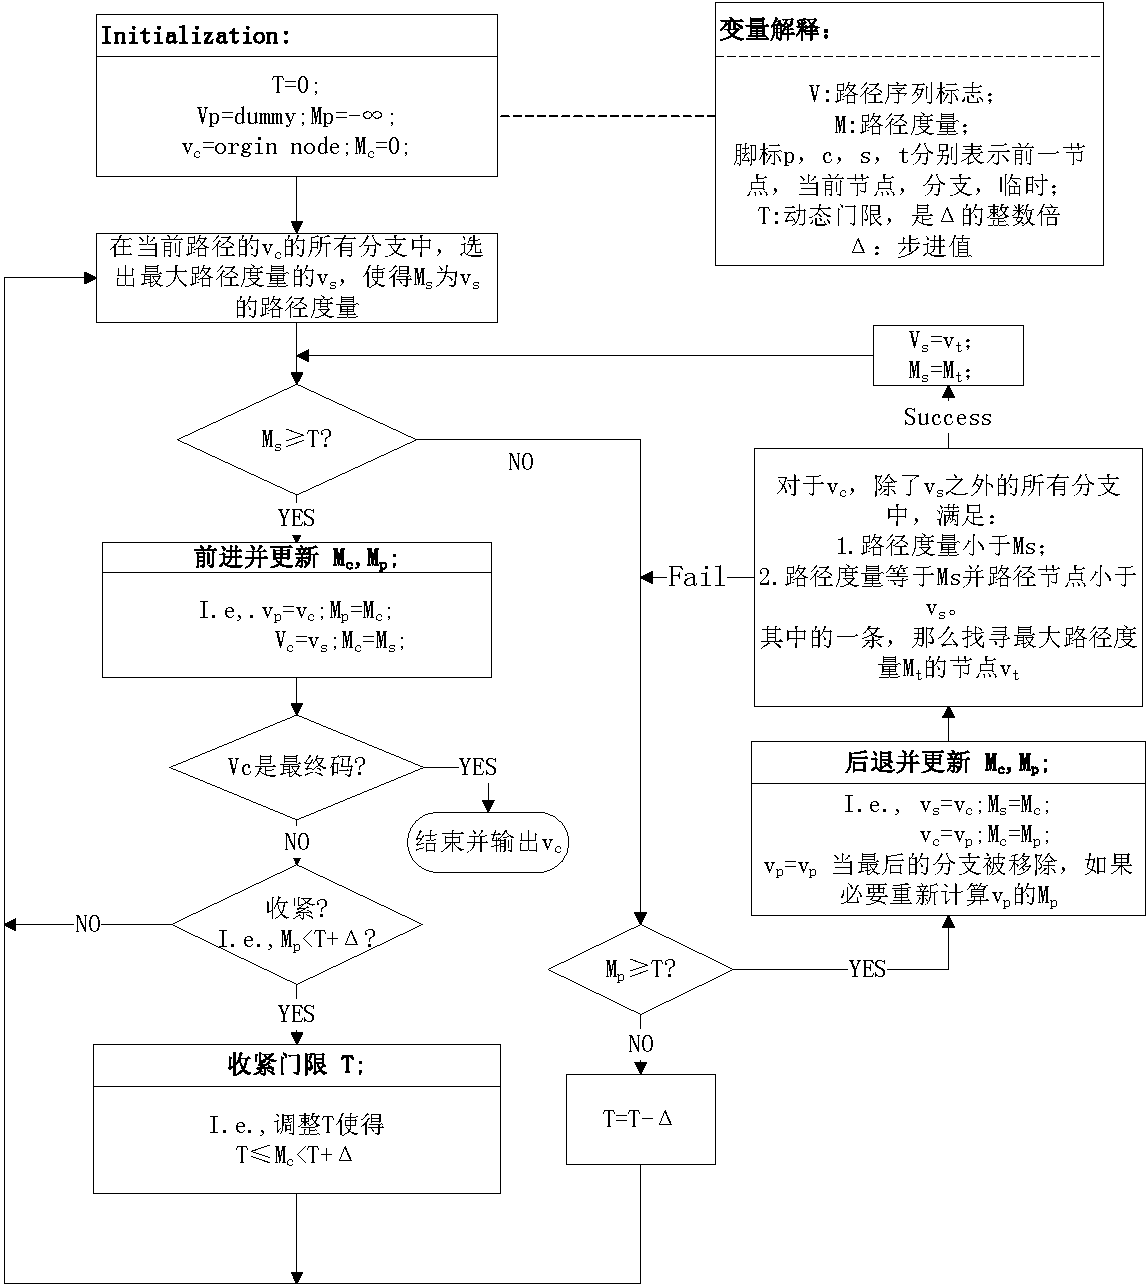
\includegraphics[width=0.8\textwidth]{images/conv5.pdf}
  \end{center}
    \caption{费诺算法流程图}
  \label{fig:3.5}
\end{figure}
结合图\ref{fig:3.5},总结费诺算法的详细步骤:
\begin{enumerate}
  \item
    初始化当前节点$v_c$为根节点,当前度量$M_c$为0,前一节点$v_p$为空,前一度量$M_p$为$-\infty$。
  \item
    在当前节点$v_c$的所有分支中,选路径度量最大的$v_s$,是的$M_s$为其路径度量。
  \item 判断$M_s\ge T$是否成立,如果否,转到第7步,如果是继续。
  \item
    路径前进一个节点,前一节点$v_p$用当前节点$v_c$代替,前一度量$M_p$由当前度量$M_c$代替;相应的,当前节点$v_c$为$v_s$,当前度量值$M_c$为$M_s$。
  \item
    判断$V_c$是否是最终码,如果是,那么结束搜索并输出$V_c$,如果不是,那么判断$M_p<T+\Delta$是否成立,如果否,跳到第2步,如果是,那么继续。
  \item 调整判决门限,是的$T\le M_c<T+\Delta$,然后继续第二步。
  \item 判断$M_p\ge
    T$是否成立,如果不成立,那么$T=T-\Delta$,如果成立,那么继续。
  \item 后退,并更新$v_c,M_c,v_p,M_p$。此过程与前进的时候相反。
  \item 如果后退成功,那么继续步骤2,否则跳到步骤7。 
\end{enumerate}
\subsection{费诺算法性能仿真}
通过matlab编程,仿真实现$K=24,R=1/2$的卷积码编译码,并画出误码率曲线,并对比在没有信道编码情况下的误码率。

仿真环境为AWGN信道,并采用BPSK调制方式。图\ref{fig:3.6}即为误码率曲线图:
\begin{figure}[htb]
  \begin{center}
    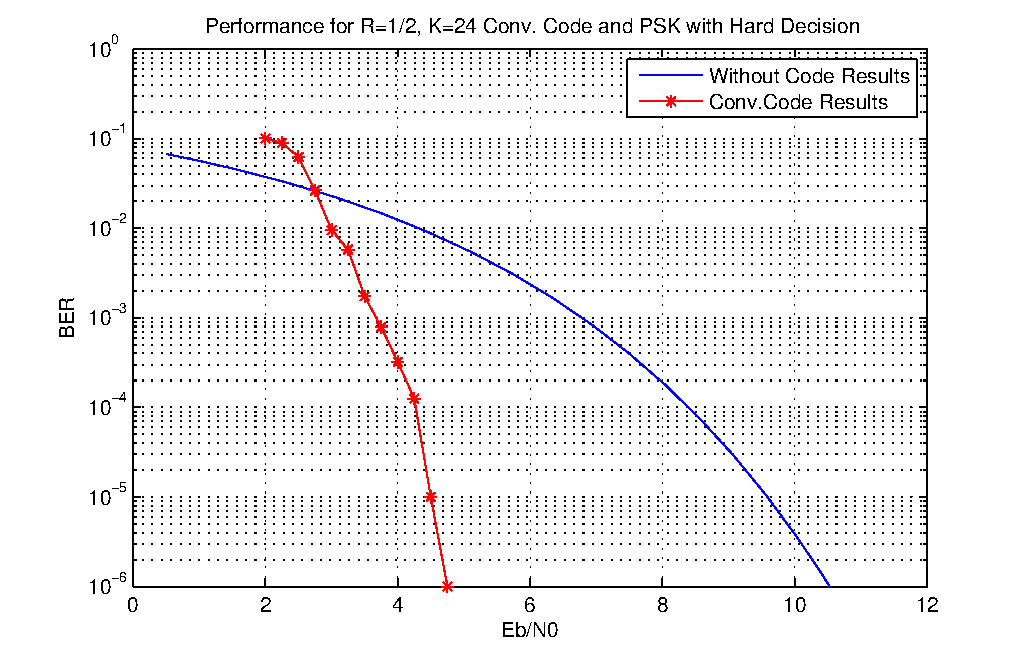
\includegraphics[width=\textwidth]{images/conv6.pdf}
  \end{center}
  \caption{误码率曲线图}
  \label{fig:3.6}
\end{figure}
图中画出误码率曲线图并对比在没有信道编码情况下的误码率,从图中可以出,卷积码编译码的误码率要比没有信道编码的好很多。图中的曲线不很平滑,可以采用差值拟合来平滑曲线。
\section{本章小结}
本章介绍了卷积码的编码与译码算法,其中着重介绍并分析了序贯译码方式,尤其是其中的费诺算法,介绍了基本原理,分析了费诺度量的计算公式及其推导过程,判决门限的作用以及步进长度$\Delta$的选取规则,用流程图详细介绍了编程实现费诺算法的步骤。并用matlab仿真,测试误码率曲线,以及参数选取是否合理。
%%========================================================================
% empty page for two-page print
\ifthenelse{\equal{\ioaside}{T}}{%
  \newpage\mbox{}%
  \thispagestyle{empty}}{}
%%========================================================================
%\end{document}
